\documentclass[../main.tex]{subfiles}
\graphicspath{{\subfix{../images/}}}
\begin{document}

A metodologia proposta neste trabalho consiste no desenvolvimento e validação de um algoritmo de otimização voltado à redistribuição de forças em veículos subaquáticos (BlueROV2), com o objetivo de manter a navegabilidade do sistema em caso de falha total de um ou mais thrusters.

Os testes serão conduzidos em ambiente de simulação, utilizando o sistema operacional Ubuntu 22.04, juntamente com o simulador Gazebo Ignition e o ROS2 control. O modelo de ROV simulado será o \textit{BlueROV2 Standard}, sendo ele utilizado para representar o comportamento dinâmico do veículo e validar o desempenho do algoritmo proposto.

A arquitetura de controle do ROV é composta por um controlador PID responsável pela estabilização da malha principal e por um controlador de alocação de esforços, responsável por distribuir as forças entre os thrusters. O algoritmo de otimização será integrado em paralelo com o controle de alocação, de modo a realizar a redistribuição adaptativa das forças quando houver falha em um ou mais propulsores. Vale destacar que o reconhecimento de falha não é abordado neste trabalho, por ser um desafio à parte da otimização das forças.

O diagrama do fluxo de controle proposto é apresentado na Figura \ref{control_logic}, ilustrando o fluxo de controle e as saídas e entradas do sistema, além de destacar a integração entre os controladores e o algoritmo de otimização. O desempenho do algoritmo será avaliado com base em dois critérios principais: a velocidade de movimentação do ROV em determinada direção e o erro de deslocamento, em caso de falha de um ou mais thrusters, para determinada direção.

\begin{figure}[H]
  \centering
  \caption{Fluxo de controle.}
  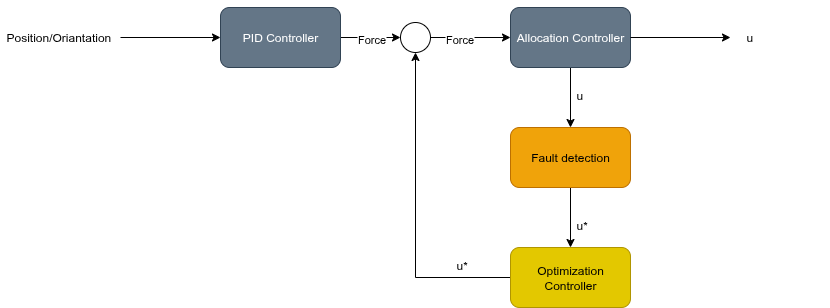
\includegraphics[width=0.7\textwidth]{images/control_logic.drawio.png}
  \vfill
  Fonte: Autores.
  % \vspace{-\baselineskip}
  \label{control_logic}
\end{figure}

A partir dessas análises é esperado verificar a robustez e a eficiência do método de otimização proposto em comparação ao controle convencional sem a tolerância a falhas.


\end{document}
